\chapter[Fundamentação Teórica]{Fundamentação Teórica}
\label{cp:fundamentacao}

\section{Gerenciamento de Projetos}

\subsection{Modelo Tradicional}

Uma metodologia de gerenciamento de projetos no modelo tradicional, de acordo com \cite{kerzner} é o alcance da excelência no gerenciamento de projetos se torna impossível sem um processo repetitivo que possa ser utilizado em cada projeto.

A gestão dos projetos segundo o \cite{pmbok}ocorre por meio de vários processos de gerenciamento, agrupados nos seguintes grupos:

\begin{itemize}
    \item Iniciação;
    \item Planejamento;
    \item Execução;
    \item Monitoramento e Controle;
    \item Encerramento.
\end{itemize}

O desenvolvimento do plano de gerenciamento do projeto é uma atividade iterativa ao longo do ciclo de vida do projeto, sempre pronto para melhoria contínua e permitindo à equipes do projeto definir e trabalhar com maior nível de detalhes. Nesta perspectiva, se tem o papel do gerente de projeto como um líder responsável por liderar a equipe para alcançar os objetivos previstos no planejamento do projeto. As principais atividades desempenhadas pelo gerente de projeto são: 

\begin{itemize}
    \item Conhecimento acerca do gerenciamento de projetos;
    \item Desempenho para aplicar seus conhecumentos na prática;
    \item Comportamento pessoal de liderança, atingindo objetivos e equilibrando restrições.
\end{itemize}

De acordo com o \cite{pmbok}, as fases são sobrepostas, ou seja, o início de uma fase é ao término de uma outra, isso leva a algumas atividades ocorrerem de forma paralela. A maneira como este tipo de projeto aumenta os riscos, retrabalhos, e exigir recursos adicionais para permitir as atividades em paralelo, como mostrado na figura \ref{img:fases_sobrepostas}.

\begin{figure}[H]
	\centering
	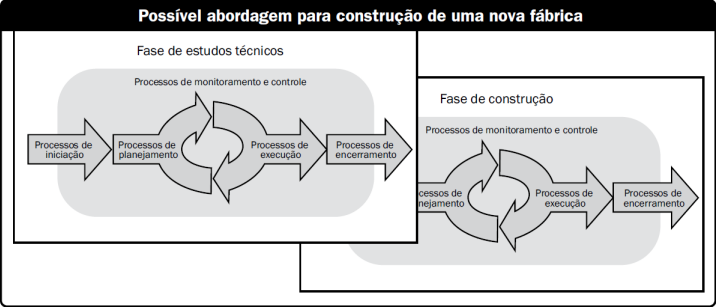
\includegraphics[width=1.0\textwidth]{figuras/fases_sobrepostas.png}
	\caption{Exemplo de projetos com fases sobrepostas. Fonte: \cite{pmbok}.}
	\label{img:fases_sobrepostas}
\end{figure}

Este tipo de gerenciamento de projeto é mais focado em empresas já consolidadas, de ramo mais formal, que possui mais burocracia em seus projetos e por tanto maior rigor de documentação e de liderança dos gerentes de projeto. Essa hierarquia pode ser vista na figura \ref{img:gerencia_de_projetos_tradicional}.

\begin{figure}[H]
	\centering
	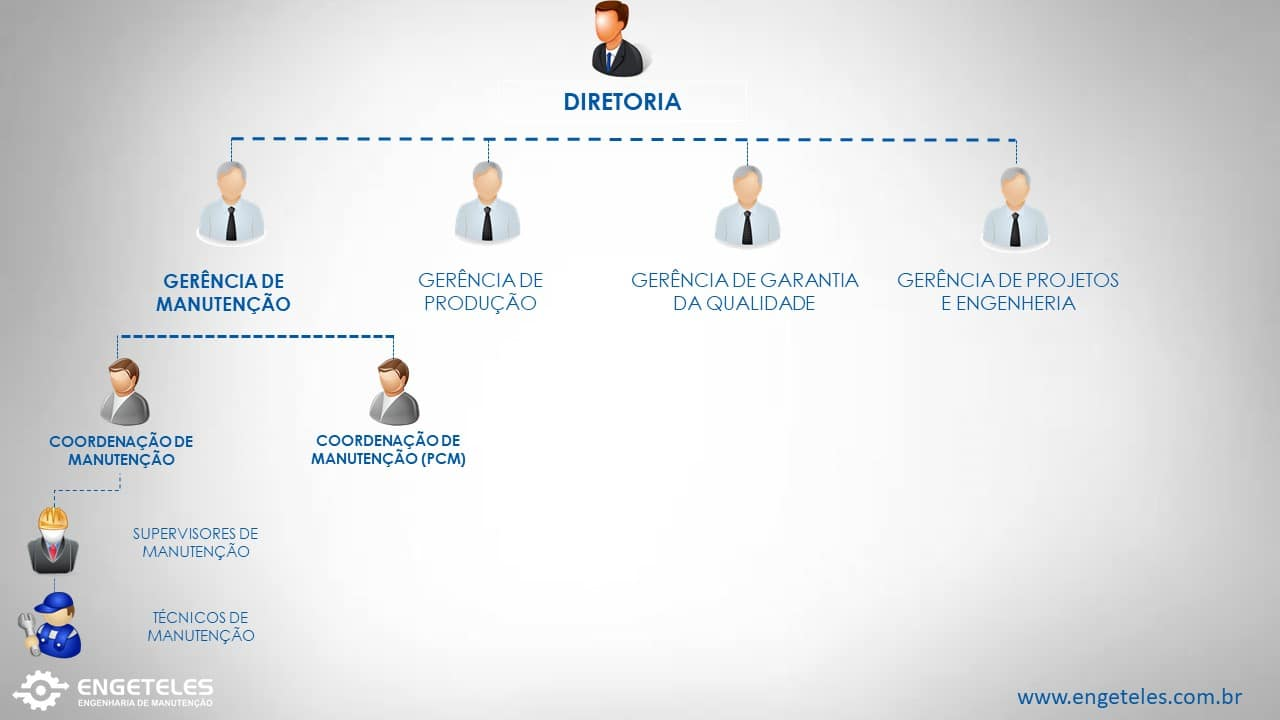
\includegraphics[width=1.0\textwidth]{figuras/gerencia_de_projeto.jpg}
	\caption{Hierarquia em projetos tradicionais. Fonte: \cite{gerentes_tradicionais}.}
	\label{img:gerencia_de_projetos_tradicional}
\end{figure}

\subsection{Modelo Ágil}

\subsection{Modelos de Reuniões}

% Tendo como premissas estes problemas, e a vontade de facilitar a operação, foram levantados a partir de estudos e dos conhecimentos adquiridos no curso de \imprimircurso uma solução que ajude gerentes e líderes de reuniões nas empresas a desenvolver encontros que sejam mais diretos e objetivos a fim de alcançar seus objetivos. Como estudo de caso foi escolhido o NMIL (Núcleo de Modernização da Informação Legislativa), um setor localizado no Senado Federal Brasileiro.

% O Senado Federal é uma instituição de âmbito nacional no Brasil, e dentre suas secretárias e setores, se tem o NMIL, o caso de estudo deste trabalho. Neste setor são realizadas reuniões quase que diariamente e a partir destes encontros podem ser gerados projetos para o próprio setor, como também para outras secretárias, então fica a cargo do NMIL realizar toda a tramitação e registrar todas as etapas. Essas informações são gravadas em papeis por vezes perdidos.

% O Sistema GRATA, vem oferecer a solução prática para a melhoria do controle das informações e qualidade dos serviços. Tendo como a principal funcionalidade o registro das Atas de reuniões de forma simples e intuitiva, tanto para quem gerencia como para quem participa. Além da automação dos processos essenciais da organização, o sistema fornece relatórios gerenciais e analíticos, que podem ser usados para identificação de pontos de melhoria ou até mesmo para dar visibilidade a questões específicas.

% \section{Reuniões Improdutivas e Suas Consequências}

% Na era do conhecimento em que estamos inseridos, reuniões estão cada vez mais presentes em organizações e segundo \cite{allen2016} essas reuniões já ocupam em média 15\% do tempo coletivo da organização. Contudo reuniões mal administradas podem levar ao desperdício de recursos da empresa, mas também a sensação dos participantes que a reunião ainda não terminou.

% O professor \cite{macleod} estima que 30\% a 60\% do tempo gasto com reuniões é desperdiçado. Gerentes podem passar por volta de 11 horas semanais com reuniões mal sucedidas, completando quase um total de 35 dias úteis ao ano. 71\% dos gerentes que foram pesquisados indicam que reuniões ineficazes os impedem de completar funções básicas em seus trabalhos, segundo \cite{perlow}.

% \textbf{COLOCAR MAIS SOBRE PROBLEMAS NO TRABALHO QUE NÃO SEJA APENAS O CUSTO}

% Uma das consequências de serem notadas em uma reunião ineficaz além de participantes dispersos e perdidos, é o custo. Estima-se que empresas gastam em média US \$ 37 bilhões anualmente em reuniões \cite{baer}. O custo real desses encontros impulsionou a \cite{harvard} a criar uma calculadora que ajuda gerentes a calcularem o verdadeiro custo de um encontro. 